%!TEX encoding = UTF-8 Unicode  
\documentclass{article}  
\usepackage{xeCJK}
\setCJKmainfont[BoldFont=STZhongsong, ItalicFont=STKaiti]{STSong}
\setCJKsansfont[BoldFont=STHeiti]{STXihei}
\setCJKmonofont{STFangsong}
\usepackage{graphicx}
\usepackage{amsmath}
\usepackage{pdfpages}
 \usepackage{clrscode}
\usepackage{listings}
\usepackage{enumerate}
\usepackage[center]{titlesec}

\lstset{language=C++}%这条命令可以让LaTeX排版时将C++键字突出显示

\lstset{breaklines}%这条命令可以让LaTeX自动将长的代码行换行排版

\lstset{extendedchars=false}%这一条命令可以解决代码跨页时,章节标题,页眉等汉字不显示的问题



\begin{document}  
\renewcommand{\contentsname}{目录}
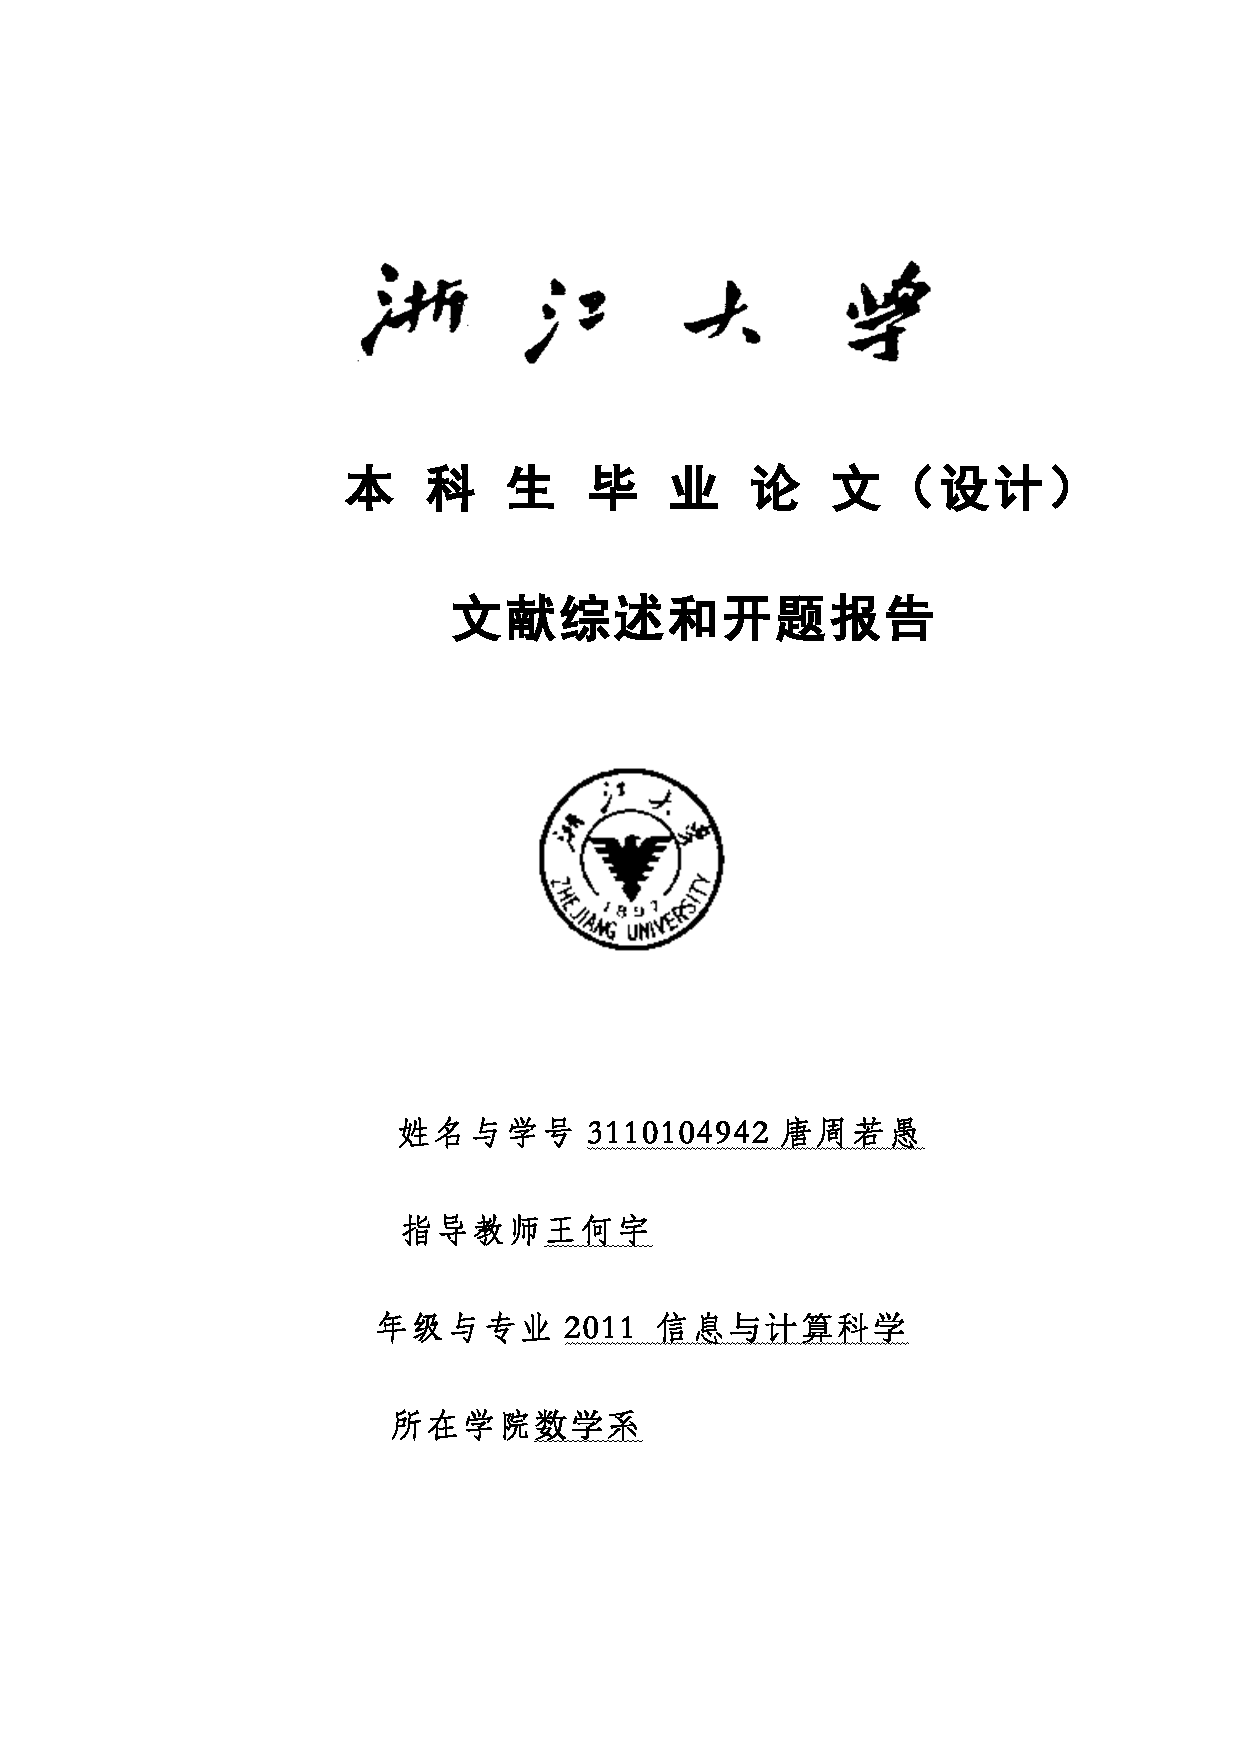
\includepdf[addtotoc={1,section,1,封面,cc},pages=1-2,offset=0cm 0.5cm]{t1.pdf}
 \tableofcontents
 \newpage
\section{开题报告}

\subsection{问题提出的背景}
    
     \subsubsection{背景介绍}
     
      近年来,在工程应用中,求解高阶矩阵的需求日益增长,全矩阵运算脱离了实际的硬件限制,为了满足这一日益增长的需求,同时这些矩阵通常都有着一个特征——非零元远少于零元,稀疏矩阵这门学科便应运而生。
在 20 世纪 60 年代研发电子网络的电子工程师们是最早的去利用稀疏性来应用稀疏矩阵进行工程上的计算的。[1]
而在微分方程数值解、线性规划等的有限元分析中,经常出现求解高阶稀疏线性方程组,如利用全矩阵进行存储,则需要$n^2$的空间复杂度和$n^3$的乘法运算时间复杂度,显然,这种程度的运算量是无法被微型计算机,甚至是工作站所接受的。
而利用矩阵的稀疏性,可以有效地减小消耗很多无谓的存储空间以及无谓的计算,在很大的程度上降低了时间和空间复杂度,降低了计算对硬件的需求,使计算成为可能。

 \subsubsection{本研究的意义和目的}

 在实际工程计算中,尤其是在微分方程数值解、线性规划等的有限元分析中,经常出现高阶的矩阵运算,经常出现百万阶、千万阶的矩阵运算,而如果使用全矩阵运算,假设是百万阶的float类型的矩阵,则需要$4*10^{12}B$来存储,也就是4TB的空间,这显然是无法被微型计算机甚至是工作站所接受的。但是通常这些矩阵具有稀疏的性质,拥有着大量的零元,而且通常阶数越高稀疏度越高。这就可以在相当大的程度上减少了存储对于硬件的压力。同时,在计算中,大量对于0的运算是五位的消耗资源的操作,也可以利用稀疏矩阵来避免这些无谓的操作。而在本研究中编写的稀疏矩阵库可以用来方便快捷的实现稀疏矩阵的存储以及一些基本运算,避免了使用者大量编写存储底层的代码,提高开发效率。
 
\subsubsection{研究现状}
在稀疏矩阵这些年的发展中,出现了很多的存储方法,比如:对角线存贮法、对称矩阵的变带宽存贮法、坐标存贮法、Elipack-Itpack存贮法、CSR存贮法、Shermans存贮法、超矩阵存贮法、动态存贮方案等。\newline
如行压缩存储方式(Compressed Row Storage):
CRS存储可以高效地存取任意一行非零元素,但存取任意一列非零元则需要遍历整个CRS存储结构。相应地,与CRS存储的稀疏矩阵相关的算法要高效的编程实现,算法的计算顺序必须按行来进行。[1]
下面对应于CRS存储:
\newline\newline\newline\newline\newline\newline\newline\newline

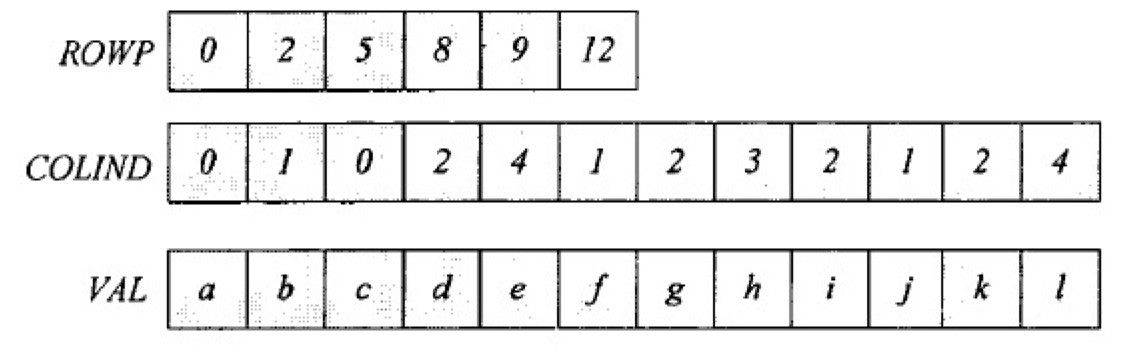
\includegraphics[scale=0.25]{crs.png} \newline
我们可以发现,ROWP数组存储的时行非零元的增长量。COLIND则存储的是列索引值,典型的C语言结构实现为\newline
\begin{lstlisting}

struct cr_matrix{ 
	int *Ri;/*col index*/ 
	int *Rp;/*length nrow+1*/ 
	double *Rx; 
	int Rncol;
	int Rnrow;
};

\end{lstlisting}
在早期计算机时,串行的算法占到主流,自然,稀疏矩阵的存储方式以及稀疏矩阵的计算都是为了串行算法服务的。但是随着计算机的发展,计算机集群、多核CPU、GPU并行等的出现,让并行算法在计算时间上远远地超越了串行算法,为了更好的适应并行计算中的稀疏矩阵计算,出现了许多新的算法以及存储方式。例如对于非结构化的矩阵,基于CUDA框架下的SCOO形式的SpMV算法比利用基于Cusp库的SCOO具有更高的效率。[2]
\newline

而在做稀疏矩阵的计算时,通常都是做一系列的基本运算,如:矩阵转置、矩阵向量乘法、矩阵矩阵乘法、数乘等。为了能得到更好的效率,许多研究者致力于寻找对于这些计算最优的存储结构及计算算法,同时提供了许多类库供科学计算使用,如:Portable, ExtensibleToolkit for Scientific Computation(PETSc)、Boost、GNU Scientific Library (GSL)等。\newline
例如,在Boost-uBLAS中有着稀疏矩阵的模板mapped\_matrix<T, F, A>(元素映射矩阵存储形式)、compressed\_matrix<T, F, IB, IA, TA>(压缩存储格式)、coordinat\_matrix<T, F, IB, IA, TA>(坐标存储格式)。
分别有着如下示例:[3]\newline
\textbf{mapped\_matrix:}
\begin{lstlisting}

#include <boost/numeric/ublas/matrix_sparse.hpp>
#include <boost/numeric/ublas/io.hpp>

int main () {
    using namespace boost::numeric::ublas;
    mapped_matrix<double> m (3, 3, 3 * 3);
    for (unsigned i = 0; i < m.size1 (); ++ i)
        for (unsigned j = 0; j < m.size2 (); ++ j)
            m (i, j) = 3 * i + j;
    std::cout << m << std::endl;
}

\end{lstlisting}

\textbf{compressed\_matrix:}
\begin{lstlisting}

#include <boost/numeric/ublas/matrix_sparse.hpp>
#include <boost/numeric/ublas/io.hpp>

int main () {
    using namespace boost::numeric::ublas;
    compressed_matrix<double> m (3, 3, 3 * 3);
    for (unsigned i = 0; i < m.size1 (); ++ i)
        for (unsigned j = 0; j < m.size2 (); ++ j)
            m (i, j) = 3 * i + j;
    std::cout << m << std::endl;
}

\end{lstlisting}

\textbf{coordinate\_matrix:}
\begin{lstlisting}

#include <boost/numeric/ublas/matrix_sparse.hpp>
#include <boost/numeric/ublas/io.hpp>

int main () {
    using namespace boost::numeric::ublas;
    coordinate_matrix<double> m (3, 3, 3 * 3);
    for (unsigned i = 0; i < m.size1 (); ++ i)
        for (unsigned j = 0; j < m.size2 (); ++ j)
            m (i, j) = 3 * i + j;
    std::cout << m << std::endl;
}
\end{lstlisting}


在多年的研究中,各种相关的研究成果页层出不穷,例如,
根据Michele Martone的研究成果,在对称矩阵乘法,或者转置的矩阵向量乘法中,RSB格式的迭代算法效率是比较高的[4]。
而在李佳佳,张秀霞,谭光明,陈明宇的研究中,得到了影响矩阵性能的参数集,可以利用该参数集提取矩阵特征,并输出最优存储格式,供数值解法器和上层应用调用。[5]
为了适用于大数据集计算以及克服现有稀疏矩阵乘法算法低效的问题,郑建华,朱 蓉,沈玉利提出了一种基于向量线性组合(VLC)的矩阵乘法处理模式,同时采用MapReduce计算模型实现了基于VLC模式的并行矩阵乘法算法。[6]
而在集群计算方面,负载平衡是不能不提到的,为了更好地发挥集群计算的计算能力,付朝江博士给出了基于贪婪分配的稀疏矩阵与向量乘的负载平衡的解决方案。[7]
\newline


\subsection{论文的主要内容和技术路线}


\subsubsection{主要研究内容} 
     在linux平台下,基于g++编译器,编写稀疏矩阵存储的C++库,实现稀疏矩阵的行压缩存储方式(Compressed Row Storage),同时实现一些稀疏矩阵的基本运算,如矩阵乘法、数乘等。为了更好地发挥CPU性能,需要实现多线程并行计算。
     
 \subsubsection{技术路线} 
 
实现稀疏矩阵的行压缩存储方式(Compressed Row Storage),通过数组存储非零元的增长量、列索引值和非零元值来实现稀疏矩阵的存储。为了实现可变长数组的存储,利用C++的STL中的vector来存储数据。
\newline
而为了更好地利用CPU的性能,利用thread库实现多线程并行计算,更为有效地利用CPU的并行性能。而为了防止多线程并行计算中“脏数据”的出现,利用mutex互斥锁保障进程安全性。
\newline
为了实现稀疏矩阵的矩阵矩阵乘法和矩阵向量乘法,可以参考全矩阵矩阵矩阵乘法和矩阵向量乘法算法,利用稀疏矩阵的零元不参与计算的特性,按照稀疏矩阵存储的结构,较全矩阵计算省略大量计算,实现稀疏矩阵计算的优势——更为高效的计算。
\newline
	

\subsubsection{可行性分析}
     \begin{enumerate}[1]
\item 	linux平台较Windows更为稳定,不容易出现宕机,且被工程界广为使用
\item 	g++是GNU的C++编译器,历史悠久,经历过多年考验,有着成熟的文档和社区帮助
\item		稀疏矩阵这门学科已存在多年,存在着成熟的存储方案及相关算法
\item		多线程的锁机制已出现多年,可以有效地保障进程安全性
\item		基于标准C++开发,有着良好的跨平台性

\end{enumerate}


\subsection{研究计划进度安排及预期目标}

      \subsubsection{进度安排}
     2014年11月24日-2014年12月21日,文献收集整理,基础知识学习。\newline
2014年12月22日-2015年1月4日,讨论算法模型,确定方案和技术路线。\newline
2015年1月5日-2015年1月29日,完成文献综述、开题报告和文献资料翻译。\newline
2015年3月9日-2015年4月5日,程序编写、调试。\newline
2015年4月6日-2015年5月3日,数值实验和数据收集。\newline
2015年5月4日-2015年5月31日,毕业论文撰写。\newline
2015年6月1日-2015年6月14日,ppt制作,准备答辩。
\newline



\subsubsection{2、预期目标}  

     利用c++在g++编译器linux平台下实现稀疏矩阵的行压缩存储方式(Compressed Row Storage)存储。可以并行计算稀疏矩阵的矩阵乘法、数乘等运算。
\newline
 
\subsection{参考文献}

  [1]张永杰、孙秦.稀疏矩阵存储技术[J].长春理工大学学报,2006年,03期:38-41.\newline
      [2]Hoang-Vu Dang,  Bertil Schmidt.CUDA-enabled Sparse Matrix–Vector Multiplication on GPUs
using atomic operations[J].Parallel Computing, 2013,Vol.39 (11):737-750.\newline
  [3]Joerg Walter and Mathias Koch.Boost 1.57.0 Library Documentation-uBLAS. http://www.boost.org/doc/libs/1\_57\_0/libs/numeric/ublas/doc/index.html, 2011\newline
  [4]Michele Martone.Efficient multithreaded untransposed, transposed or symmetric sparse matrix–vector multiplication with the Recursive Sparse Blocks format[J].Parallel Computing, 2014,40:47-58.\newline
  [5]李佳佳,张秀霞,谭光明,陈明宇.选择稀疏矩阵乘法最优存储格式的研究[J].计算机研究与发展 , Journal of Computer Research and Developmen,2014年,04期:882-894.\newline
  [6]郑建华,朱 蓉,沈玉利.Sparse matrix multiplication algorithm based on MapReduce[J].仲恺农业工程学院学报,2013年,03期:45-50.\newline
[7]付朝江.基于贪婪分配的稀疏矩阵与向量乘的负载平衡[J].福建工程学院学报 ,2010年,01期:79-82.
 \newpage
\section{文献综述}
\subsection{背景介绍}

      近年来,在工程应用中,求解高阶矩阵的需求日益增长,全矩阵运算脱离了实际的硬件限制,为了满足这一日益增长的需求,同时这些矩阵通常都有着一个特征——非零元远少于零元,稀疏矩阵这门学科便应运而生。
在 20 世纪 60 年代研发电子网络的电子工程师们是最早的去利用稀疏性来应用稀疏矩阵进行工程上的计算的。[1]
而在微分方程数值解、线性规划等的有限元分析中,经常出现求解高阶稀疏线性方程组,如利用全矩阵进行存储,则需要$n^2$的空间复杂度和$n^3$的乘法运算时间复杂度,显然,这种程度的运算量是无法被微型计算机,甚至是工作站所接受的。
而利用矩阵的稀疏性,可以有效地减小消耗很多无谓的存储空间以及无谓的计算,在很大的程度上降低了时间和空间复杂度,降低了计算对硬件的需求,使计算成为可能。

\subsection{国内外研究现状}
\subsubsection{研究方向及进展}

在这些年的发展中,出现了很多的存储方法,比如:对角线存贮法、对称矩阵的变带宽存贮法、坐标存贮法、Elipack-Itpack存贮法、CSR存贮法、Shermans存贮法、超矩阵存贮法、动态存贮方案等[2]。
\newline
如行压缩存储方式(Compressed Row Storage):
CRS存储可以高效地存取任意一行非零元素,但存取任意一列非零元则需要遍历整个CRS存储结构。相应地,与CRS存储的稀疏矩阵相关的算法要高效的编程实现,算法的计算顺序必须按行来进行。[3]
下面对应于CRS存储:
\newline\newline\newline\newline\newline\newline\newline

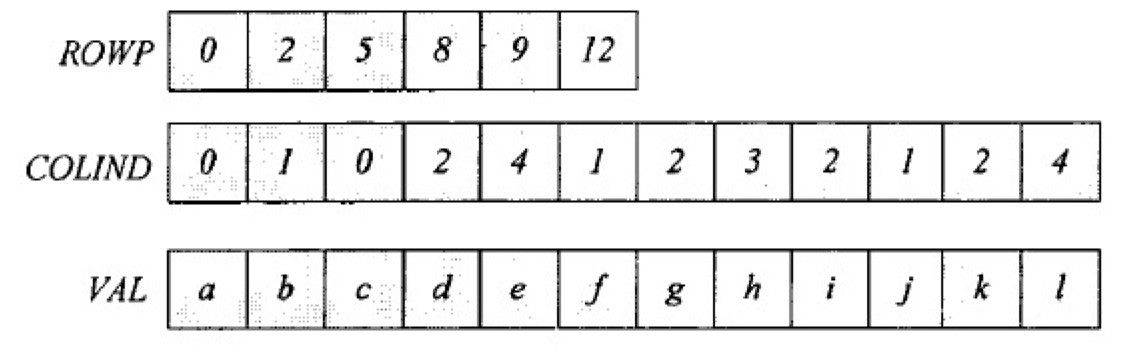
\includegraphics[scale=0.25]{crs.png}
我们可以发现,ROWP数组存储的时行非零元的增长量。COLIND则存储的是列索引值,典型的C语言结构实现为\newline

\begin{lstlisting}

struct cr_matrix{ 
	int *Ri;/*col index*/ 
	int *Rp;/*length nrow+1*/ 
	double *Rx; 
	int Rncol;
	int Rnrow;
};

\end{lstlisting}


在早期计算机时,串行的算法占到主流,自然,稀疏矩阵的存储方式以及稀疏矩阵的计算都是为了串行算法服务的。但是随着计算机的发展,计算机集群、多核CPU、GPU并行等的出现,让并行算法在计算时间上远远地超越了串行算法,为了更好的适应并行计算中的稀疏矩阵计算,出现了许多新的算法以及存储方式。例如对于非结构化的矩阵,基于CUDA框架下的SCOO形式的SpMV算法比利用基于Cusp库的SCOO具有更高的效率。[4]
\newline
而在做稀疏矩阵的计算时,通常都是做一系列的基本运算,如:矩阵转置、矩阵向量乘法、矩阵矩阵乘法、数乘等。为了能得到更好的效率,许多研究者致力于寻找对于这些计算最优的存储结构及计算算法,同时提供了许多类库供科学计算使用,如:Portable, ExtensibleToolkit for Scientific Computation(PETSc)、Boost、GNU Scientific Library (GSL)等。\newline
例如,在Boost-uBLAS中有着稀疏矩阵的模板mapped\_matrix<T, F, A>(元素映射矩阵存储形式)、compressed\_matrix<T, F, IB, IA, TA>(压缩存储格式)、coordinat\_matrix<T, F, IB, IA, TA>(坐标存储格式)。
分别有着如下示例:[5]\newline
\textbf{mapped\_matrix:}
\begin{lstlisting}

#include <boost/numeric/ublas/matrix_sparse.hpp>
#include <boost/numeric/ublas/io.hpp>

int main () {
    using namespace boost::numeric::ublas;
    mapped_matrix<double> m (3, 3, 3 * 3);
    for (unsigned i = 0; i < m.size1 (); ++ i)
        for (unsigned j = 0; j < m.size2 (); ++ j)
            m (i, j) = 3 * i + j;
    std::cout << m << std::endl;
}

\end{lstlisting}

\textbf{compressed\_matrix:}
\begin{lstlisting}

#include <boost/numeric/ublas/matrix_sparse.hpp>
#include <boost/numeric/ublas/io.hpp>

int main () {
    using namespace boost::numeric::ublas;
    compressed_matrix<double> m (3, 3, 3 * 3);
    for (unsigned i = 0; i < m.size1 (); ++ i)
        for (unsigned j = 0; j < m.size2 (); ++ j)
            m (i, j) = 3 * i + j;
    std::cout << m << std::endl;
}

\end{lstlisting}

\textbf{coordinate\_matrix:}
\begin{lstlisting}

#include <boost/numeric/ublas/matrix_sparse.hpp>
#include <boost/numeric/ublas/io.hpp>

int main () {
    using namespace boost::numeric::ublas;
    coordinate_matrix<double> m (3, 3, 3 * 3);
    for (unsigned i = 0; i < m.size1 (); ++ i)
        for (unsigned j = 0; j < m.size2 (); ++ j)
            m (i, j) = 3 * i + j;
    std::cout << m << std::endl;
}
\end{lstlisting}

在多年的研究中,各种相关的研究成果页层出不穷,例如,
根据Michele Martone的研究成果,在对称矩阵乘法,或者转置的矩阵向量乘法中,RSB格式的迭代算法效率是比较高的[6]。
而在李佳佳,张秀霞,谭光明,陈明宇的研究中,得到了影响矩阵性能的参数集,可以利用该参数集提取矩阵特征,并输出最优存储格式,供数值解法器和上层应用调用。[7]
为了适用于大数据集计算以及克服现有稀疏矩阵乘法算法低效的问题,郑建华,朱 蓉,沈玉利提出了一种基于向量线性组合(VLC)的矩阵乘法处理模式,同时采用MapReduce计算模型实现了基于VLC模式的并行矩阵乘法算法。[8]
而在集群计算方面,负载平衡是不能不提到的,为了更好地发挥集群计算的计算能力,付朝江博士给出了基于贪婪分配的稀疏矩阵与向量乘的负载平衡的解决方案。[9]
\newline

\subsubsection{存在问题}

稀疏矩阵的存储没有一种通用的形式,各种形式都各有利弊[10],这也就需要我们对于不同的情况去寻找最合适的存储形式来计算,虽然李佳佳,张秀霞,谭光明,陈明宇[7]的研究得到了一个参数集用以寻找最优存储形式,但是比较的存储形式比较少,还有多种形式没有计入考量范围。
\newline
而在超大规模的稀疏矩阵计算时,计算机的内存可能不能完全存储这些数据,部分数据将会存储在硬盘中,而硬盘的读取效率远低于内存,如何更好地将硬盘中的数据读取到内存中,减少内存与硬盘交互的时间,同时,如何降低内存与缓存间的交互时间也是一个问题。
\newline
而随着计算机的普及,计算机进入了家家户户,分布式计算逐渐成为可能,让普通的计算机使用者参与到科学计算中,贡献GPU资源来帮助研究人员更快地完成计算,但是这尚未得到普及,同时,中国尚未形成一个成熟的分布式计算平台,也没有培养出普通用户参与到分布式计算项目的习惯。\newline



\subsubsection{研究展望}
为了更好的适应现代的工程计算需求,计算更大规模的稀疏矩阵,以及适应新的CPU指令集和GPU计算框架,稀疏矩阵的存储形式值得进一步的研究。同时,伴随着分布式计算的发展,更为高效的冗余计算机制和任务分配机制也将会带给稀疏矩阵计算新的研究方向。
按照摩尔定律,计算机的计算能力将毎隔18-24个月翻一番,那么计算稀疏矩阵的能力也将相应提高。同时随着量子计算机、光计算机等的出现,更高德计算能力也将随之到来。而为了更好地发挥这些硬件的能力,以往的算法可能并不再适合了,需要开发新的算法以适应新的硬件。而对于硬件商而言,如Intel、AMD等CPU厂商而言,封装更多的CPU指令,让用户可以直接调用CPU指令来进行科学计算,更好地发挥硬件的性能。对于普通计算机用户,培养参与到分布式计算的习惯,通过建立一个国家级的分布式计算中心,建立奖励机制,鼓励普通计算机用户参与到分布式计算中,为研究计划中的稀疏矩阵计算贡献自己的计算资源。\newline

\subsection{参考文献}
      \qquad
\newline
 [1]Yousef Saad.Iterative Methods for Sparse Linear Systems[M].SECOND EDITION.USA:Society for Industrial and Applied Mathematics,2003年.68.\newline
 [2]张永杰、孙秦.稀疏矩阵存储技术[J].长春理工大学学报,2006年,03期:38-41.\newline
 [3]冯广祥. 大型稀疏矩阵直接求解算法的研究及实现[8].  东北大学:系统工程,2010.\newline
    [4]Hoang-Vu Dang,  Bertil Schmidt.CUDA-enabled Sparse Matrix–Vector Multiplication on GPUs
using atomic operations[J].Parallel Computing, 2013,Vol.39 (11):737-750.\newline
 [5]Joerg Walter and Mathias Koch.Boost 1.57.0 Library Documentation-uBLAS. http://www.boost.org/doc/libs/1\_57\_0/libs/numeric/ublas/doc/index.html, 2011\newline
  [6]Michele Martone.Efficient multithreaded untransposed, transposed or symmetric sparse matrix–vector multiplication with the Recursive Sparse Blocks format[J].Parallel Computing, 2014,40:47-58.\newline
  [7]李佳佳,张秀霞,谭光明,陈明宇.选择稀疏矩阵乘法最优存储格式的研究[J].计算机研究与发展 , Journal of Computer Research and Developmen,2014年,04期:882-894.\newline
  [8]郑建华,朱 蓉,沈玉利.Sparse matrix multiplication algorithm based on MapReduce[J].仲恺农业工程学院学报,2013年,03期:45-50.\newline
[9]付朝江.基于贪婪分配的稀疏矩阵与向量乘的负载平衡[J].福建工程学院学报 ,2010年,01期:79-82.\newline
[10]张永杰,孙秦.稀疏矩阵存储技术[J].长春理工大学学报,2006年,03期:38-41.\newline
 



 \newpage
\section{文献翻译}
\subsection{原文}
\qquad
\newline
\includepdf[addtotoc={1,section,1,title in toc,cc},pages=81-94,offset=0cm 0.5cm]{saad.pdf}


\subsection{译文}
\qquad
\newline


就像在上一节描述的一样,标准的离散化的偏微分方程往往会伴随着一个庞大的且稀疏的矩阵。稀疏矩阵可以被模糊的描述为一个具有非常少的非零元的矩阵。但是,事实上,当特殊的技巧需要利用到大量的非零元以及它们的位置时,一个矩阵是可以被稀疏化的。这些稀疏化矩阵的技巧是从不储存零元的想法开始的。一个关键的问题是制定能够适合于高效地使用不论是直接还是迭代的标准计算方法的存储稀疏矩阵的数据结构。这一章节将简介稀疏矩阵,它们的属性、呈现,以及用以存储它们的数据结构。
\newline\newline

\subsection*{3.1介绍}

利用一个矩阵中的零元以及它们的位置的自然的想法最初是由在不同学科的工程师们提出的。在涉及带状矩阵的简单地例子中,特殊的技巧直接的被发明了。在20世纪60年代研发电子网络的电子工程师们是最早的去利用稀疏性来对于具有特殊结构的矩阵解决一般稀疏线性系统。对于稀疏矩阵技巧而言,最主要也是最早需要解决的问题是去设计一个在线性系统中得直接求解算法。这些算法需要是可以接受的,在存储和计算效率上。直接的稀疏算法可以被用于计算那些庞大的难以被稠密算法来实现的问题。
\newline\newline\newline\newline\newline\newline\newline\newline

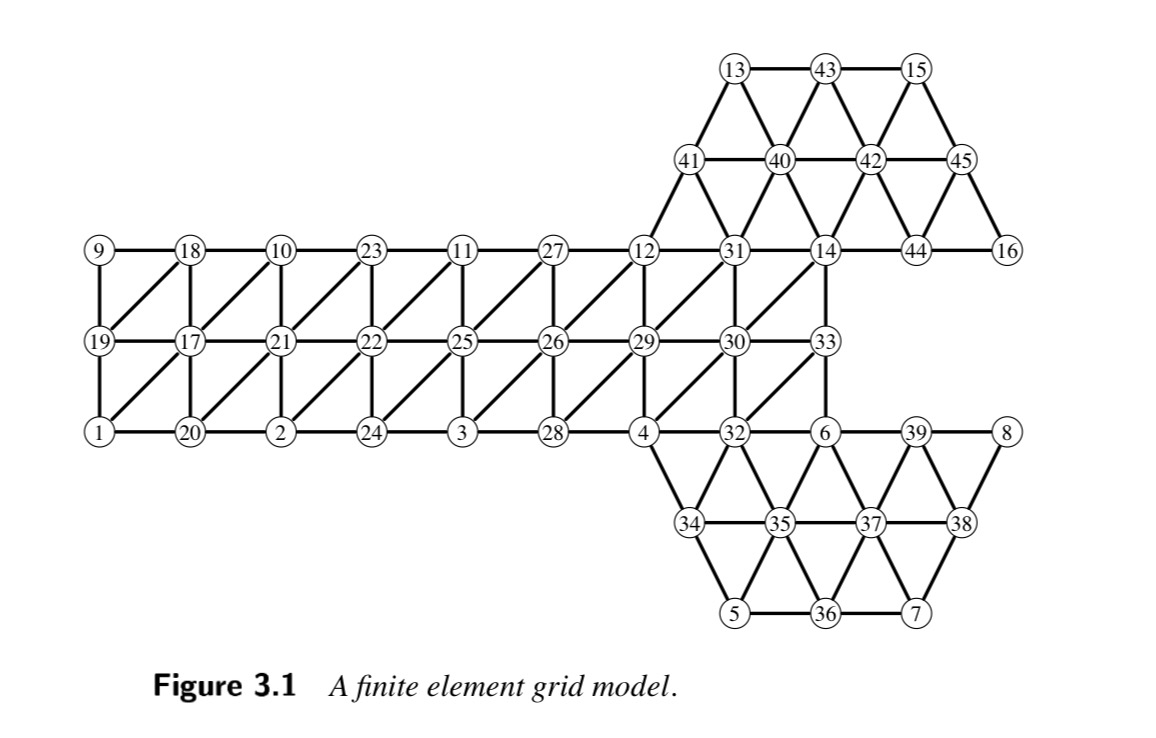
\includegraphics[scale=0.25]{3_1.png}

基本上,有两个明显的类别的稀疏矩阵,结构化的和非结构化的。一个结构化的矩阵是指一个非零元的位置形成某个规律的矩阵,通常这些非零元在对角线附近。要不然,这些非零元会在相同大小的块内(稠密子矩阵),而这也会形成一个规律,通常这些非零元在对角线(块)附近。一个具有着不规则位置的非零元的矩阵会被称作是非结构化的。最好的一个结构化的矩阵的例子是一个只有着少量对角元的矩阵。网格上的有限差分矩阵,就像上一节中提到的,是典型的具有着规律结构的例子。大部分的对于复杂几何的有限元和有限体积技巧会导致非结构化的矩阵。图3.2展示了一个与图3.1所呈现的有限元网格问题的一个小规模的非结构化的矩阵。
\newline

这两种类型的矩阵间的区别可能并不会明显的影响到直接求解技巧,而且,在过去,它并没受到过多的关注。但是,对于迭代求解方法,这个区别是很重要的。在这些方法中,最基本的运算之一是矩阵向量求积。在高性能计算机上,这些运算受规则化程度的影响很大。比如,在向量计算机上,理想的是存储对角元,但是更通常的设计可能会较慢,因为他们需要间接寻址。
\newline

下一节将讨论用图来呈现稀疏矩阵。
\newline\newline\newline\newline\newline\newline
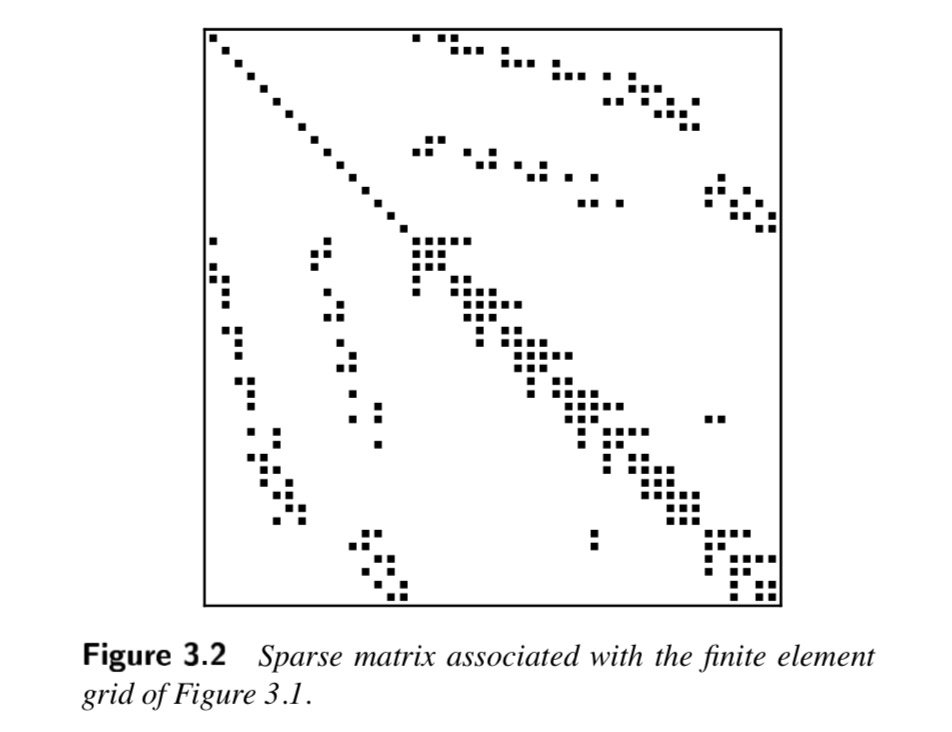
\includegraphics[scale=0.4]{3_2.png}
\newline\newline
\subsection*{3.2图论}

图论是用来表示稀疏矩阵结构的一个理想的工具,因此,在稀疏矩阵技巧中,它扮演着一个主要的角色。例如,图论是用于解决并行稀疏高斯消除和预处理技术的关键。在下一节中,将讨论图的一般特性,以及它们在有限元和有限差分矩阵中得应用。
\newline
\subsection*{3.2.1图与邻接图}
记住一个图由两个集合定义,一个顶点集合$V =\{v_1,v_2,\cdots,v_n\}$和一个边的集合E,E是由点对$(v_i,v_j)$组成的,$v_i,v_j$都是V中的元素,换而言之,$E\subseteq V\times V$。这个图$G=(V,E)$通常被平面内的一系列的被边联系的点的向量来表示。这个图被用来描述集合V中元素间的关系。例如,V可以被用来描述世界上的主要城市。线就是两个城市间的直达航线。那么这个图就会描述这样一个关系“在城市A和城市B间存在一条直达航线”。在这个特殊的例子中,二元关系很可能是对称的,换而言之,如果有一条A到B的直达航线,那么也有一条B到A的直达航线。在这样的情形中,图被称作是无向的,用以与通常的有向图相对。
  \newline\newline\newline\newline\newline\newline\newline\newline\newline
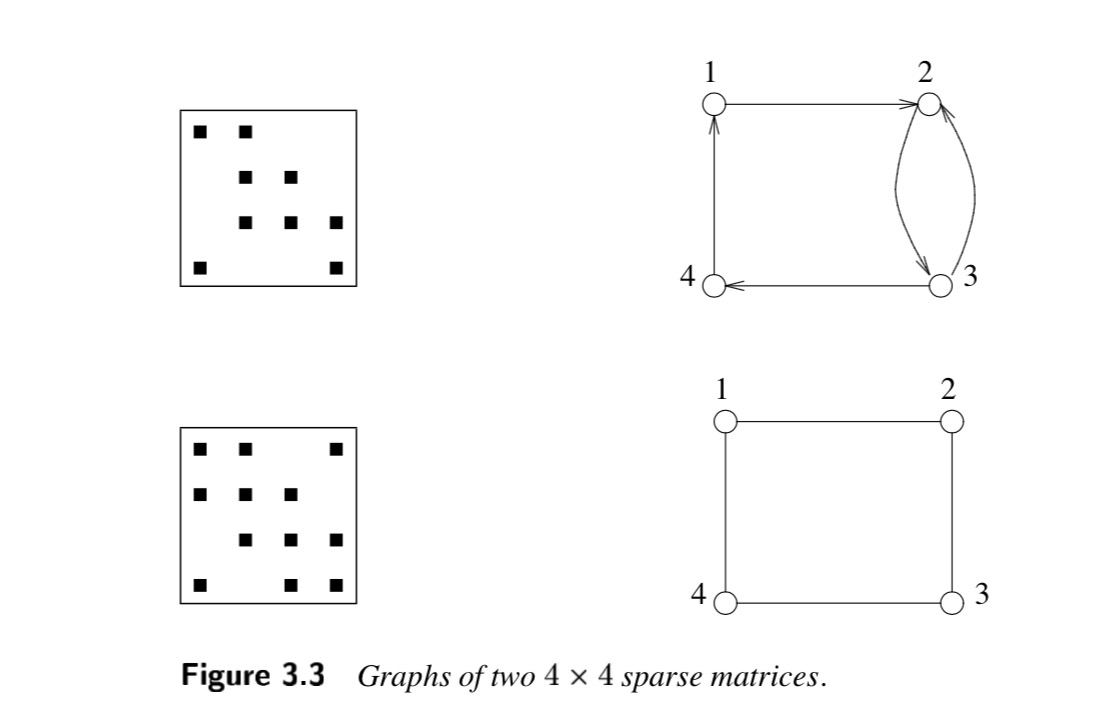
\includegraphics[scale=0.25]{3_3.png}
\newline\newline
回到稀疏矩阵,稀疏矩阵的邻接图是一个图$G=(V,E)$,V中得n个顶点代表n个未知数。它的边是按照以下规则建立的方程式建立的二元关系:当$a_{ji}\neq0$时,有一条从节点i指向节点j的边。而这条边将因此描述包含未知量j的二元关系方程式i。注意,这个图是有向的,除非这个矩阵是有对称结构的(对任意的$1\leq i,j\leq n$,若$a_{ji}\neq 0$,那么$a_{ij}\neq 0$ )。
\newline
当一个矩阵的非零元总有一个对称非零元,换而言之$a_{ij}$和$a_{ji}$总是同时为非零元,那么这图就是无向的。因此,对于无向图,每条边都有两个方向。因此,无向图可以用无向边来表现。
\newline
作为利用图模型的例子,并行高斯消去法可以通过寻找在指定消去阶段的未知数来获得。根据以上的二元关系,这些未知数两两独立。这些与未知数一致的行可以被用作基。因此,在一个极端情况下,当一个矩阵是对角阵,那么所有的未知数是独立的。与之相反的是,当一个矩阵是稠密的,那么每一个未知量都与其他未知量相关。稀疏矩阵则介于这两种极端情况之间。
\newline
邻接图有一些有趣的简单性质。$A^2$的图可以被解释成一个n顶点图,对每条边的点对(i,j), 表示在原图A中至少存在一条长度确切的说是2的从节点i到节点j的路径。与之相似的时,$A^k$的图包含的时用以描述从节点i到节点j的至少存在一条长度为k的路径的二元关系的边。欲知详情,请看练习4.
\newline
\subsection*{3.2.2PDE矩阵的图}

对于在每个网格点只涉及一个屋里未知量的偏微分方程,离散矩阵的邻接图通常就是用来描述网格的图。但是,在每个网格点上有着多个未知量是很常见的。例如,模拟流体流动的方程可能涉及流体的两个速度分量(二维)以及在每个网格点的能量和动量。在这样的情况下,有两种用来标记未知量的选择。在每个网格点,它们可以被连续的标记。因此,在刚才的例子中,我们可以在一个指定的网格点例如u(k),$\cdots$,u(k+3)上标记所有的四个未知量(两个速度的分量,动量以及压力)。另外,所有的与一类变量相关的未知量可以最先被标记(比如,第一个速度分量),接下来是第二类的变量(比如,第二个速度分量)等等。在任意情况下,很明显邻接矩阵是有冗余信息的。物理网格的商图可以被用来替代使用。这将节约大量的存储量和计算量。在上述的流体流动的例子中,用以描述图的整数数组的存储可以被缩小到接近1/16。这是因为边的数量被所见到了大约这么多,但是通常很小的顶点数却保持着不变。
\newline
\subsection*{3.3置换和重新排序}

对于稀疏矩阵而言,重排序行或列,或者行和列是一个常见操作。事实上,重排序行和列是一个用于直接求解法和迭代法并行实现的一个最重要的部分。本节介绍这些重排技术和矩阵的邻接图的相关思想的关系。记得在第一章中,矩阵的第j列记作$a_{*j}$,第i行则记作$a_{i*}$。
\newline
\subsection*{3.3.1基础概念}

我们先开始一个定义与符号。
\newline
\textbf{定义3.1}有一个矩阵A,以及$\pi =\{i_1,i_2,\cdots ,i_n\}$的一个交换集合$\pi =\{i_1,i_2,\cdots ,i_n\}$。那么矩阵$$A_{\pi ,*}=\{ a_{\pi(i),j} \}_{i=1,\cdots ,n;j=1,\cdots ,m},$$
$$A_{*,\pi }=\{i, a_{\pi(j)} \}_{i=1,\cdots ,n;j=1,\cdots ,m}$$就分别被称作A的行$\pi$-交换和列$\pi$-交换。
\newline
广为周知的时,最多n个交换(换而言之,就是只互换两项的基本排列)可以产生集合$\{1,2,\cdots,n\}$的任意置换。一个交换矩阵就是一个两行互换了得单位矩阵。用$X_{ij}$来表示第i和j行交换了的单位矩阵。注意到,为了交换矩阵A的第i和j行,我们可以用矩阵$X_{ij}$来左乘矩阵A。让$\pi=\{i_1,i_2,\cdots,i_n\}$为一个任意序列。这个置换就是一系列连续的交换矩阵$\sigma(i_k,j_k),k=1,\cdots,n$的乘积。那么,我们就可以通过交换矩阵的$i_1$和$j_1$行,然后再结果矩阵的基础上交换$i_2$和$j_2$行,以此类推,最后交换$i_n$和$j_n$行。每一步我们都可以通过左乘矩阵$X_{i_k,j_k}$来实现。同样的,对于矩阵的列也是一样的:为了交换矩阵的第i和k列,通过右乘矩阵$X_{i_k,j_k}$可以实现。从上我们可以得到下述命题。
\newline
\textbf{命题3.1}让$\pi$是交换$\sigma(i_k,j_k),k=1,\cdots,n$的乘积得到的置换。那么,$A_{\pi,*}=P_{\pi}A$,$A_{*,\pi}=AQ_{\pi}$,当


\begin{equation}
P_{\pi}=X_{i_n,j_n}X_{i_{n-1},j_{n-1}}\cdots X_{i_1,j_1}  \tag{3.1}
\end{equation}
\begin{equation}
Q_{\pi}=X_{i_1,j_1}X_{i_{2},j_{2}}\cdots X_{i_n,j_n} \tag{3.2}
\end{equation}

这些交换矩阵的乘积被称作置换矩阵。显然,一个置换矩阵只不过是进行了行列交换的单位矩阵。
\newline
注意到$X_{i,j}^2=I$,换而言之,置换矩阵的平方是一个单位矩阵,或者等价地,置换矩阵的逆等于它本身,这是很显然的一个属性。易见,矩阵(3.1)和(3.2)满足
$$P_{\pi}Q_{\pi}=X_{i_n,j_n}X_{i_{n-1},j_{n-1}}\cdots X_{i_1,j_1}\times X_{i_1,j_1}X_{i_2,j_2}\cdots X_{i_n,j_n}$$表示了矩阵$Q_{\pi}$和$P_{\pi}$都是非退化的,且互为另一个的逆。换而言之,用同一个置换矩阵来交换一个矩阵的行和列事实上做了类似的变换。因为定义(3.1)和(3.2)中得$P_{\pi}$和$Q_{\pi}$的乘积是相反的顺序,另一个推论就显而易见了。由于每一个基矩阵$XX_{i_k,j_k}$是对称的,那么$Q_{\pi}$是$P_{\pi}$的转置。因此$$Q_{\pi}=P_{\pi}^T=P_{\pi}^{-1}$$
因为矩阵$P_{\pi}$的逆矩阵是它的转置,置换矩阵就是唯一的。
\newline
另一个用来推出上述关系的方法是用置换矩阵$P_{\pi}$和$P_{\pi}^T$来代表行列交换了的单位矩阵。(在练习3中)显而易见$$P_{\pi}=I_{\pi,*},P_{\pi}^T=I_{*,\pi}$$
那么,接下来就可以直接验证$$A_{\pi,*}=I_{\pi,*}A=P_{\pi}A,A_{*,\pi}=AI_{*,\pi}=AP_{\pi}^T$$
这对于在线性系统中解释置换操作很重要。当矩阵的行交换了,方程的顺序就改变了。换而言之,当列交换了,那么未知量就会对应的改变标记或者改变顺序。
\newline
\textbf{例子3.1}思考,比如,线性系统$Ax=b$,当
$$
A=
\left (                 
\begin{array}{cccc}   
    a_{11} & 0 & a_{13} & 0\\  
    0 & a_{22} & a_{23} & a_{24} \\ 
    a_{31} & a_{32} & a_{33} & 0 \\ 
    0 & a_{42} & 0 & a_{44} \\ 
\end{array}
\right)                
$$
以及$\pi = \{1,3,2,4\}$,那么(列)交换线性系统是
$$
\left (                 
\begin{array}{cccc}   
    a_{11} & a_{13}& 0 & 0\\  
    0 & a_{23}& a_{22}  & a_{24} \\ 
    a_{31} & a_{33}& a_{32}  & 0 \\ 
    0  & 0& a_{42} & a_{44} \\ 
\end{array}
\right)          
\left (                 
\begin{array}{c}   
    x_{1} \\  
    x_{2} \\  
    x_{3} \\  
    x_{4} \\  
\end{array}
\right)           
=
\left (                 
\begin{array}{c}   
    b_{1} \\  
    b_{2} \\  
    b_{3} \\  
    b_{4} \\  
\end{array}
\right)   
$$
注意到,不只是未知量交换了,方程也是,特别的,右边没有变。
\newline
在上述例子中,只有A的列交换了。在稀疏矩阵技术中,这样的单侧变换不如两侧变换寻常。事实上,这通常与线性系统中得对角元起着一个明显且重要的角色的事实有关。比如,在偏微分应用中,对角元通常很大,而且,在交换矩阵中可能很需要去保留这一性质。为了达到这一目的,很典型的是去同时对A的行和列进行相同的交换。这样的操作被叫做对称置换,若果用$A_{\pi,\pi}$来表示,那么,这样的对称置换的结果就满足这一关系
$$A_{\pi,\pi}=P_{\pi}^TAP_{\pi}$$
对称置换的解释很简单。由此产生的矩阵用相同的方式重命名,或重标记,或重排序未知量和重排序等式。
\newline
\textbf{例子3.2}
对于前面的例子,如果行和列用相同的置换矩阵来置换,那么线性系统可以这样来获得
$$
\left (                 
\begin{array}{cccc}   
    a_{11} & a_{13}& 0 & 0\\  
     a_{31} & a_{33}& a_{32}  & 0 \\ 
    0 & a_{23}& a_{22}  & a_{24} \\ 
    0  & 0& a_{42} & a_{44} \\ 
\end{array}
\right)          
\left (                 
\begin{array}{c}   
    x_{1} \\  
    x_{2} \\  
    x_{3} \\  
    x_{4} \\  
\end{array}
\right)           
=
\left (                 
\begin{array}{c}   
    b_{1} \\  
    b_{2} \\  
    b_{3} \\  
    b_{4} \\  
\end{array}
\right)   
$$
注意到,对角元是原来的矩阵的对角元在主对角线上德一个不一样的顺序。
\newline

\subsection*{3.3.2与邻接图的关系}
从图论的角度,另一个对于对称置换的重要解释是这相当于不不改变边来重新标记顶点。事实上,(i,j)是原矩阵A的邻接图的边,A'是交换了得矩阵。当且仅当$(\pi(i),\pi(j))$是原始矩阵A的图中的一条边时,那么$a_{ij}'=a_{\pi(i),\pi(j)}$,结果(i,j)是交换了的矩阵A'的邻接图中一条边。因此,交换了的矩阵的图没有改变;甚至,顶点的标记也是。与之相对的是,不对称置换就不会保存好图。事实上,它们可以将一个无向图转换为一个有向图。尽管邻接矩阵的一般图是相同的,对称置换可能会对矩阵的结构造成一些重大的影响。
\newline
\textbf{例子3.3}考虑图3.4描述的矩阵和它的邻接图。因为它们的形状,这样的矩阵又是被叫做“箭头”矩阵,但是,因为它们图的结构可能更适合把它们叫做“星”矩阵。
\newline
如果用置换$9,8,\cdots,1$来重排序等式,图3.5所描述的矩阵和图就得到了。尽管两张土建的区别看起来很小,但是矩阵可能会有一个对于算法有着重要影响的完全不同的结构。以此为例,如果用高斯消去法来重排序矩阵,那么填充就不会发生。换而言之,LU分解的L和U部分会与A的下和上两部分有着一样的结构。在另一方面,在原始矩阵上作高斯消去法会导致灾难性的填充。特别的,在高斯消去法第一部以后,LU分解的L和U部分是稠密矩阵。用直接稀疏矩阵技术,找到在高斯消去过程中对于较少填充有作用的矩阵的置换很重要。
\newline
最后这一段,总的来说,两侧非对称置换也可能在实践中出现。然而,在直接法中它们很常见。
\subsection*{3.3.3常用重排序}
在
实践中,重排序和置换的种类七绝与直接或者迭代法是否被考虑。下面是一个这样的对赌迭代法更为有用的一个重排序的例子。
\newline\newline\newline\newline\newline\newline\newline\newline
\newline\newline\newline\newline\newline\newline
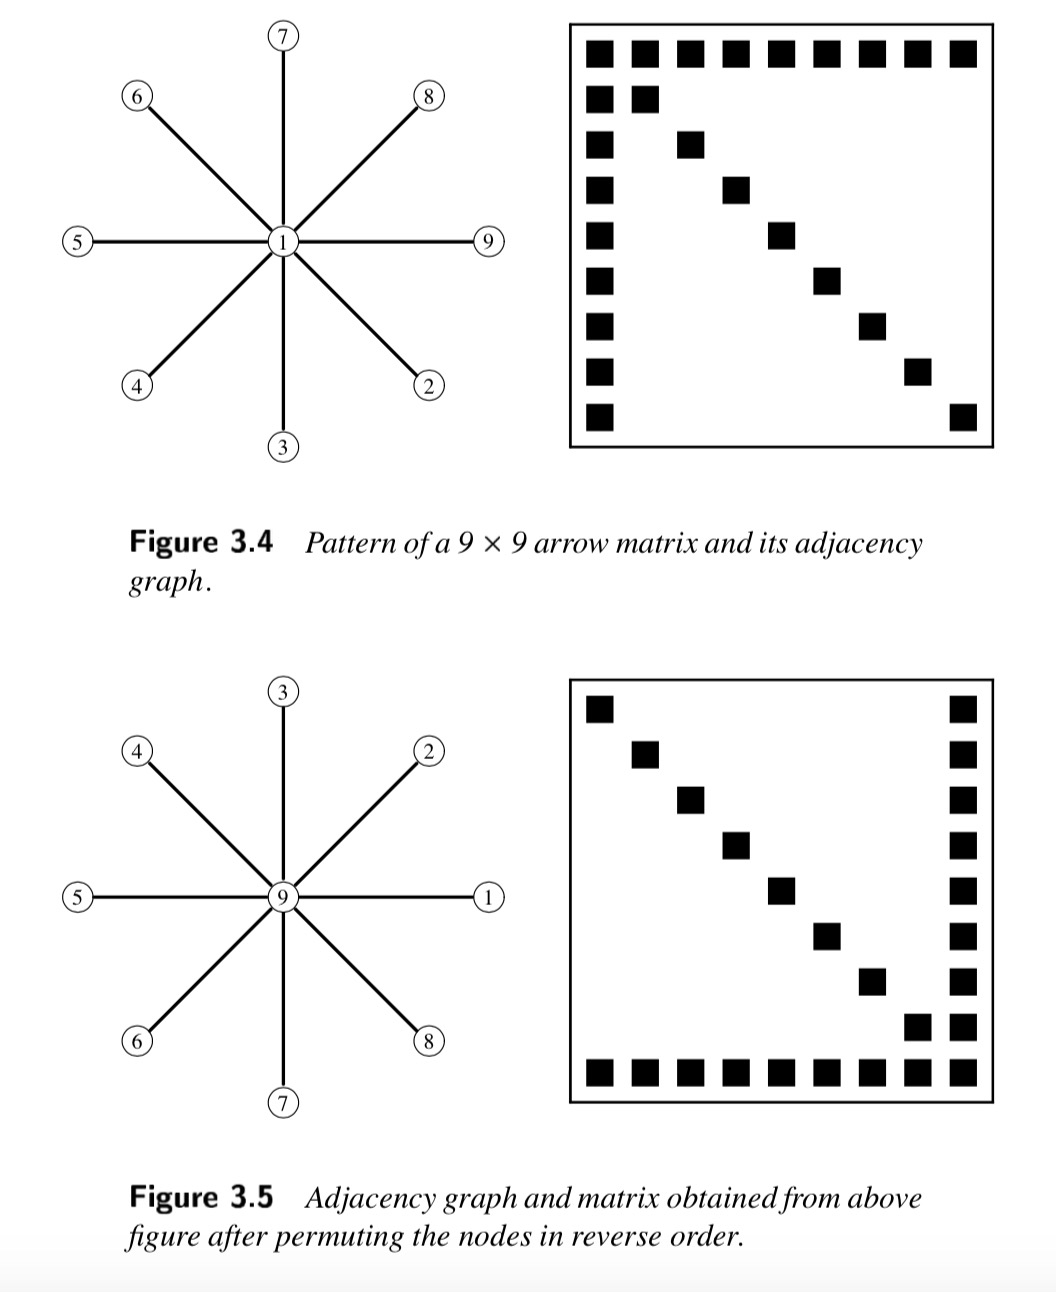
\includegraphics[scale=0.25]{3_4_5.png}

\textbf{水平集序}这种顺序类型包含了许多基于水平集的图的便利的技巧。水平集是递归定义的上一级的所有节点的所有未标记的邻集。最初,一个水平集有一个节点,虽然有几个将来会被讨论的也重要的起始点。当一个水平集被遍历完成,它的节点就被标记了且排了编号。比如,它们可以按照遍历的顺序来编号。另外,遍历顺序的不同会产生不同的顺序。例如,某一个水平集中的节点可以按照它们列出的自然序访问。然后,可以检查它们每一个的邻节点。每一次,当遇到一个访问过的顶点有一个没有编号的邻节点,那么它就被添加到列表中并标记为下一水平集的下一元素。在图论中,这个简单地策略被称为广度优先搜索。在每个水平集中,顺序取决于节点遍历的方式。在广度优先搜索中,水平集中元素总是以它们列出的自然序来遍历。在Cuthill-McKee排序中,水平集的元素被以从最低到最高的顺序来遍历。


\includepdf[addtotoc={1,section,1,title in toc,cc},pages=3-3,offset=0cm 0.5cm]{t1.pdf}


\end{document}  
